\subsection{User}

\begin{figure}[H]
\centerline{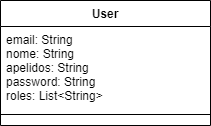
\includegraphics[width=4cm]{figuras/diseño/User.png}}
\caption{Documento User.}
\label{enlaceUser}
\end{figure}

La \hyperref[enlaceUser]{Figura 3.8} ilustra las características del documento {\it User} de la aplicación. Está formado por los siguientes atributos:

\begin{itemize}
    \item {\bf email}: Correo electrónico del usuario.
    \item {\bf nome}: Nombre del usuario.
    \item {\bf apelidos}: Apellidos del usuario.
    \item {\bf password}: Contraseña del usuario. Se almacena encriptada.
    \item {\bf roles}: Roles del usuario. Solo existen dos posibles valores: ``ROLE\_USER'' y ``ROLE\_ADMIN''.
\end{itemize}